\chapter{Collider Phenomenology}
In this chapter, we will discuss how to connect theory and experiment. We will begin by connecting scattering amplitudes and physically observed cross sections, after which we will briefly discuss detector components of the LHC, and then move on to the question of how we establish statistical significance given experimental data from detectors.
% Scattering amplitudes and cross sections\\
\section{Detector design for hadron colliders}
Particle colliders can broadly be classified as lepton or hadron colliders. Each one has its advantages and disadvantages. Lepton colliders have cleaner signals than hadron colliders due to the lack of large QCD backgrounds. On the other hand, hadron colliders are able to reach much larger center-of-mass energies. This is because leptons, when forced along a circular path, lose large amounts of energy via synchrotron radiation.

We will first begin by describing the components of a generic detector at a hadron collider. At the Large Hadron Collider at CERN, the two major experiments are ATLAS (A Toroidal LHC Apparatus) and CMS (Compact Muon Solenoid). The detectors used by these experiments differ slightly in construction, but essentially probe the same physics. A cutaway view of the ATLAS detector is shown in \label{fig:ATLAS_cutaway}.

\begin{figure}[h]
  \begin{sidecaption}
    { Cutaway view of the ATLAS detector, showing the various components. Taken from \citep{Atlas2008}.}
    \centering
  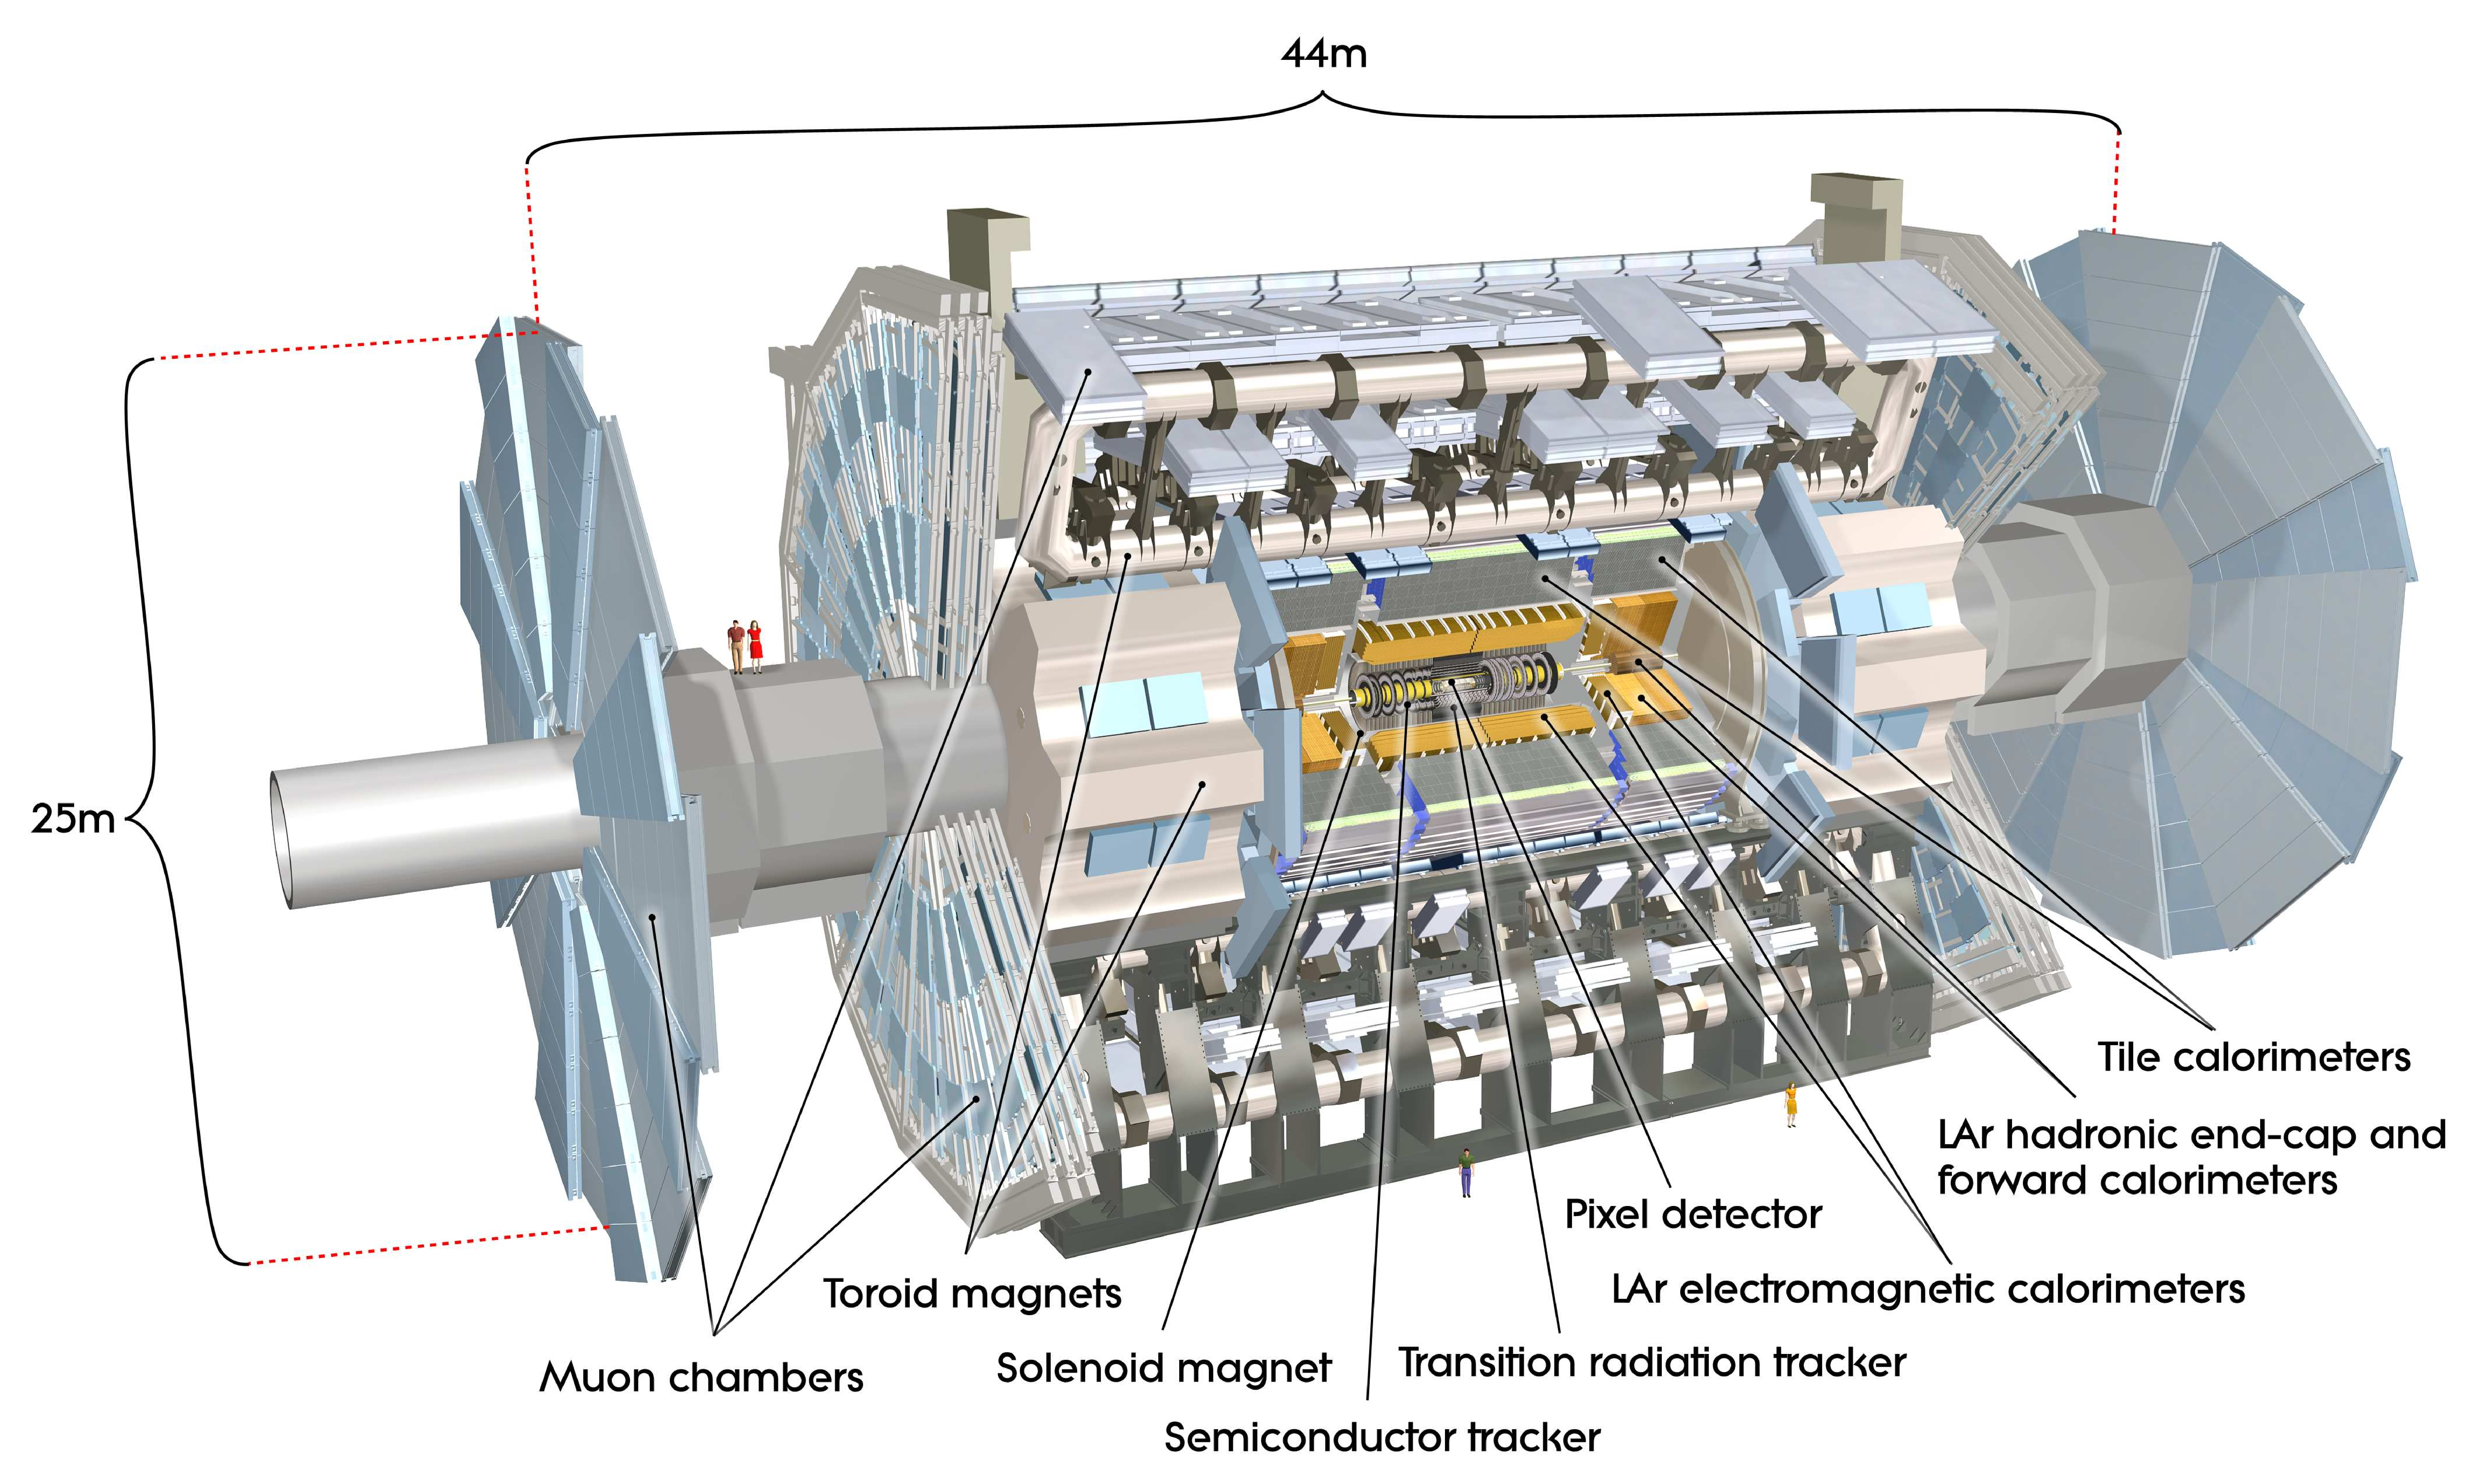
\includegraphics[trim = {2cm 5cm 2cm 2cm}, clip, width=1\textwidth]{images/atlas}
  \end{sidecaption}
  \label{fig:ATLAS_cutaway}
\end{figure}

\paragraph{Tracking chamber}
\paragraph{Electromagnetic calorimeter}
\paragraph{Hadronic calorimeter}
\paragraph{Muon chambers} The muon is able to penetrate through the other layers.

\section{Future circular colliders}

\begin{figure}[h]
  \begin{sidecaption}
    {Schematic diagram of the FCC ring. Tunneling under Lake Geneva will be a major challenge for the construction of the ring.}
    \centering
  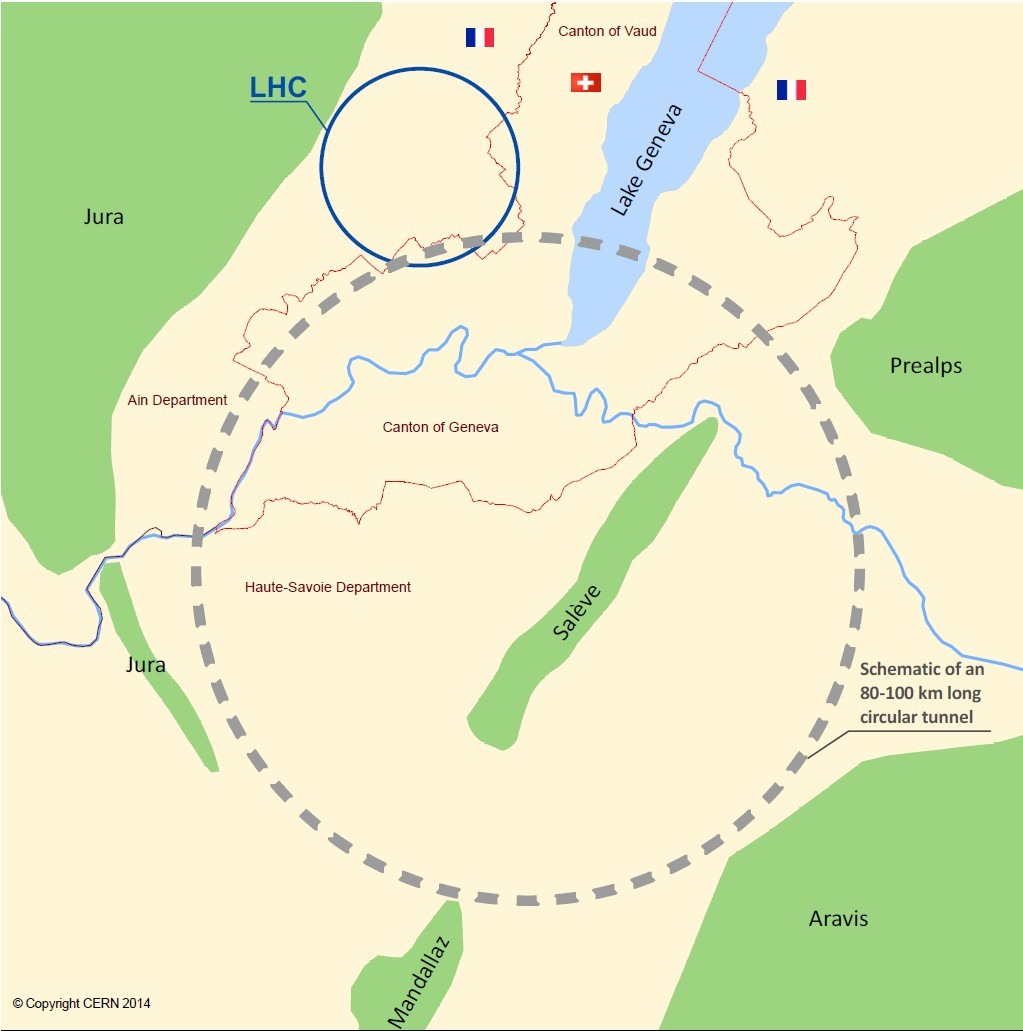
\includegraphics[width=0.9\textwidth]{images/FCC_ring_schematic}
  \end{sidecaption}
\end{figure}
\section{Anatomy of a collider analysis}
\subsection{Monte Carlo simulations}
\subsection{Showering and hadronization}
\subsection{Detector simulation and reconstruction}
\section{Statistical significance in particle physics}
